\chapter{Introdução}

\section{Contexto}

Medir a qualidade do código-fonte  de um software é um processo fundamental no seu desenvolvimento, pois daí surgem indicadores sobre os efeitos que uma alteração no código irá causar ou sobre os efeitos gerados na qualidade do software após a adesão de uma nova prática na equipe de desenvolvimento \cite{Fenton98}. 

Como a qualidade do código fonte está relacionada à qualidade interna do produto de software \cite{ISO25023}, sua medição, e consequentemente as melhorias implantadas nele afetam a qualidade do produto como um todo. Do ponto de vista da engenharia de software, métricas de código fonte de um software fornecem uma maneira quantitativa de avaliar a qualidade de atributos internos do produto, habilitando assim a avaliação da qualidade antes do produto ser concluído \cite{pressman_engenharia_2010}.

Além disso, o processo de medição da qualidade interna do software possibilita também não só entender e controlar o que está se passando no seu desenvolvimento, como também ser encorajado a tomar decisões que visem a sua melhoria \cite{Fenton98}.
 
\section{Problema}
\label{intro_problema}

Apesar de métricas de código-fonte serem coletadas facilmente com o auxílio de ferramentas de análise estática de código, como, por exemplo, por meio do \textit{Sonar} e o \textit{Analizo}, sua interpretação ainda pode ser um desafio que se não for superado pode tornar essa coleta algo sem muito valor observável. Ferramentas de análise de métricas frequentemente exportam seu resultado como valores numéricos isolados \cite{Meirelles2013} e, segundo \citeonline{marinescu2005measurement}, a utilização de métricas isoladas dificulta a interpretação de anomalias do código, reduzindo a aplicabilidade da medição feita. Além disso, o autor ainda afirma que a métrica por si só não contém informação suficiente para motivar uma transformação no código que que melhore sua qualidade. 

A dificuldade em interpretar os dados disponibilizados por tais ferramentas de análise do código afeta a avaliação de projetos de software, onde são um fator essencial para a tomada de decisão à nível de gerenciamento de projeto, de processo, de engenharia de software e de outros processos de apoio \cite{pandian_software_2004}. Surge a partir desse fato a necessidade de uma solução que apoie a tomada de decisão, associando esses valores numéricos à uma semântica de interpretação como cenários de limpeza. Cenários de limpeza fazem parte de um conceito levantado através do mapeamento desenvolvido por \cite{Machini2010}, que se baseou em conceitos teóricos focados nos trabalhos de \citeonline{Martin2008} e \citeonline{Beck2007}. 

Buscando facilitar a interpretação das métricas de código fonte, bem como apoiar as decisões de refatoração a serem tomadas, \citeonline{rego_monitoramento_2014} construiu uma solução que faz uso de um ambiente de DW para armazenamento e monitoramento de métricas. Dá-se então a necessidade de investigar, por meio de estudo de caso, a eficácia e eficiência da solução de DW proposta no contexto do problema descrito. Assim foi criada a seguinte questão geral de pesquisa:

\textit{O uso de um ambiente de Data Warehousing para aferição e monitoramento da qualidade interna do código-fonte é eficaz e eficiente do ponto de vista da equipe de qualidade?}


\section{Objetivos}

O objetivo geral deste trabalho consiste na análise da eficácia e eficiência do uso de \textit{Data Warehousing} no monitoramento de métricas de código fonte. Como este trabalho é dividido em duas partes, seus objetivos também foram divididos dessa forma, sendo os objetivos da primeira parte, são:

\begin{easylist}[itemize]	
	
	& levantar fundamentação teórica que servirá de base para todo o trabalho;
	& analisar solução desenvolvida por \citeonline{rego_monitoramento_2014} para monitoramento de métricas por meio de um ambiente de \textit{Data Warehousing}; e
	& definir, projetar e caracterizar o do estudo de caso.
	
	
	\end{easylist}	

A segunda parte deste trabalho, a ser desenvolvida no primeiro semestre de 2015, terá os seguintes objetivos:	

\begin{easylist}[itemize]	
	
	& realizar um estudo com uso de estatística descritiva para analisar o comportamento da taxa de oportunidade de melhoria de código-fobte, apresentada na solução. Espera-se identificar com esse estudo, padrões, tendências e possivelmente, valores de referência para interpretação desse indicador;
	& coletar os dados que surgirão como respostas das questões específicas elaboradas para o estudo de caso, como por exemplo o nível de satisfação quanto ao uso da solução ou qual a taxa de oportunidade de melhoria de código em um determinado intervalo de tempo.
	& coletar dados de um projeto em desenvolvimento na organização selecionada;
	& realizar análise dos dados coletados.
	& relatar resultados obtidos.
	
	\end{easylist}

\section{Metodologia de Pesquisa}

Nessa seção será definida a metodologia da pesquisa, definindo qual a natureza da pesquisa, a forma de abordagem, o tipo de objetivo que se espera alcançar, os procedimentos técnicos e o tipo de coleta de dados. A figura \ref{fig:metodologiadepesquisa} apresenta um esquema para a metodologia, buscando classificar a pesquisa quanto aos elementos que a classificam segundo \citeonline{metodologia_edna}:

\begin{figure}[h!]
\centering
\includegraphics[keepaspectratio=false,scale=0.40]{figuras/figuras_matheus/metodologia_da_pequisa.eps}
\caption{Metodologia de pesquisa}
\label{fig:metodologiadepesquisa}
\end{figure}
\FloatBarrier

Do ponto de vista da natureza, uma pesquisa pode ser considerada básica ou aplicada \cite{metodologia_edna}. A pesquisa a qual esse trabalho se refere é aplicada pois seus resultados contém aplicação prática e são dirigidos à solução de problemas específicos.

A abordagem da pesquisa será tanto qualitativa quanto quantitativa, pois ao mesmo tempo em que busca classificar informações em números através de técnicas estatísticas, também analisa a subjetividade de algumas questões sem que isso seja traduzido em números.

O objetivo que essa pesquisa busca alcançar faz com que ela seja considerada descritiva, pois uma pesquisa descritiva visa descrever as características de determinado fenômeno envolvendo uso de técnicas padronizadas de coleta de dados \cite{metodologia_edna}. Quanto aos procedimentos técnicos ela pode ser considerada de levantamento, pois envolve a interrogação direta das pessoas cujo comportamento se deseja conhecer. Além disso, do ponto de vista dos procedimentos técnicos, ela também pode ser considerada bibliográfica, documental e como um estudo de caso.

Também foi modelado no esquema da metodologia quais serão as formas de coleta de dados. Como pode pode ser visto na figura \ref{fig:metodologiadepesquisa}, a coleta é feita através de questionários, obervação na vida real e documentos, que incluem o próprio relatório da solução adotada no estudo de caso.

As etapas necessárias para o desenvolvimento do projeto de estudo de caso se baseiam na diagramação de pesquisa de \citeonline{gil_como_2002}, nos passos para elaborar um estudo de caso elicitados por \citeonline{yin2001estudo} e no protocolo de estudo de caso de \citeonline{case-study-template-2008}. A figura \ref{fig:projeto-pesq} apresenta os elementos do projeto com sua ordem de execução em forma de fluxo.


% @Figure projeto-pesq
\begin{figure}[h!]
\centering
\includegraphics[keepaspectratio=false,scale=0.65]{figuras/figuras_pedro/projeto-pesq.eps}
\caption{Diagramação do projeto de estudo de caso}
\label{fig:projeto-pesq}
\end{figure}
\FloatBarrier


Os passos específicos do estudo de caso são apresentados após a identificação do tipo de pesquisa. Assim a partir do passo de determinação do plano até o passo de seleção da amostra são apresentados o projeto de estudo de caso onde serão identificados elementos como o problema a ser resolvido, a questão de pesquisa e demais tópicos definidos no protocolo de estudo de caso. Em seguida, a coleta de dados é feita através de questionários, entrevistas informais, observações em campo e resultados provenientes da solução de DWing que será utilizada. A etapa de análise e interpretação dos dados  refere-se às atividades de categorização, exibição, verificação e conclusão de dados de natureza qualitativa e quantitava. Por fim, a redação do relatório de pesquisa apresenta a redação dos resultados de forma adequada para o leitor alvo.



\section{Organização do Trabalho}

Este trabalho está dividido em 5 capítulos:

	\begin{easylist}[itemize]	
	
	& \textbf{Capítulo 1 - Introdução:} Esse capítulo tem como objetivo apresentar o contexto que esse trabalho está inserido, o problema sobre o qual ele buscará resolver, qual a justificativa e os objetivos da sua realização e como essa pequisa foi elaborada.
	& \textbf{Capítulo 2 - Métricas de Software:} Capítulo responsável pela explicação teórica a respeito do que são métricas de código e como elas foram utilizadas no desenvolvimento da solução que esse trabalho busca analisar.
	& \textbf{Capítulo 3 - Data Warehouse:} Nesse capítulo serão apresentados conceitos teóricos sobre \textit{Data Warehousing}, assim como a maneira como foi desenvolvido o ambiente de \textit{Data Warehouse} para armazenamento de métricas de código fonte.
	& \textbf{Capítulo 4 - Projeto de estudo de caso:} Será apresentada a estratégia de pesquisa adotada durante o trabalho, buscando elaborar um protocolo para o estudo de caso que será realizado. Elementos de pesquisa como o problema a ser resolvido, os objetivos a serem alcançados no estudo de caso e quais os métodos de coleta e análise dos dados serão identificados e explicados.
	& \textbf{Capítulo 5 - Conclusão:} Além das considerações finais dessa primeira parte do trabalho, serão descritos objetivos para a segunda parte a ser realizada ao término desta.
	
	\end{easylist}	
